% Template LaTeX source file for homework problem solutions.
% Alan T. Sherman (9/9/98)

% Running LaTeX
%
% Name this file FOO.tex
% latex FOO
% latex FOO   
%    (You have to run latex twice to get the cross references correct.
%     Running latex creates a file FOO.dvi 
%     You can view dvi files with the program xdvi )
% xdvi FOO.dvi &
%
% lpr -d FOO.dvi
%    (To print the dvi file.   Be sure to use the "-d" print option,
%     and be sure your printer can handle dvi files (not all printers can).
%     Do NOT print with "lpr FOO.dvi", which will print tens of pages
%     of unreadable dvi source code. Printing a postscript (ps) file
%     is usually more reliable, as explained below.)
%
% dvips FOO.dvi
%    (To create a postscript file named FOO.ps 
%     which you can view with the program ghostview )
% ghostview FOO.ps &
% lpr FOO.ps
%    (To print the ps file.)

%%%%%%%%%%%%%%%%%%%%%%%%%%%%%%%%%%%%%%%%%%%%%%%%%%%%%%%%%%%%%%%%%%%%%%

\documentclass[12pt]{article}
\usepackage{amsmath,amssymb,graphicx}

% Set the margins
%
\setlength{\textheight}{8.5in}
\setlength{\headheight}{.25in}
\setlength{\headsep}{.25in}
\setlength{\topmargin}{0in}
\setlength{\textwidth}{6.5in}
\setlength{\oddsidemargin}{0in}
\setlength{\evensidemargin}{0in}




%%%%%%%%%%%%%%%%%%%%%%%%%%%%%%%%%%%%%%%%%%%%%%%%%%%%%%%%%%%%%%%%%%%%%%%
% Macros

% Math Macros.  It would be better to use the AMS LaTeX package,
% including the Bbb fonts, but I'm showing how to get by with the most
% primitive version of LaTeX.  I follow the naming convention to begin
% user-defined macro and variable names with the prefix "my" to make it
% easier to distiguish user-defined macros from LaTeX commands.
%
\newcommand{\myN}{\hbox{N\hspace*{-.9em}I\hspace*{.4em}}}
\newcommand{\myZ}{\hbox{Z}^+}
\newcommand{\myR}{\hbox{R}}

\newcommand{\myfunction}[3]
{${#1} : {#2} \rightarrow {#3}$ }

\newcommand{\myzrfunction}[1]
{\myfunction{#1}{{\myZ}}{{\myR}}}


% Formating Macros
%

\newcommand{\myheader}[4]
{\vspace*{-0.5in}
\noindent
{#1} \hfill {#3}

\noindent
{#2} \hfill {#4}

\noindent
\rule[8pt]{\textwidth}{1pt}

\vspace{1ex} 
}  % end \myheader 

\newcommand{\myalgsheader}[0]
{\myheader{METU, Computer Engineering}
{CENG564 - Pattern Recognition THE "2" \\ "{\bf Deniz Rasim Uluğ}"  - "2172088" "{\bf Kaan Hamilton}"  - "2035962"} {Fall 2016}{}}

% Running head (goes at top of each page, beginning with page 2.
% Must precede by \pagestyle{myheadings}.
\newcommand{\myrunninghead}[2]
{\markright{{\it {#1}, {#2}}}}




%%%%%% Begin document with header and title %%%%%%%%%%%%%%%%%%%%%%%%%

\begin{document}

\myalgsheader
\pagenumbering{gobble}
\pagestyle{plain}



\section*{Questions} 

% fill the blanks with your answers
\section*{Answer 1}
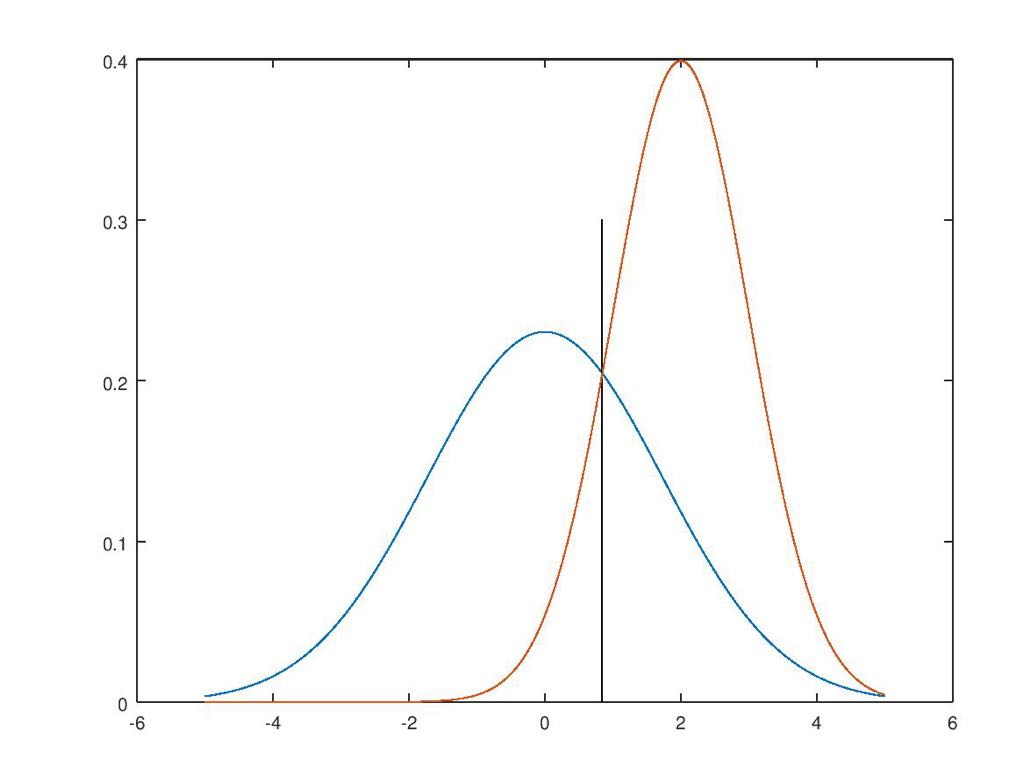
\includegraphics[scale=0.35]{q1.jpeg}

 a) The likelihood ratio is $\frac{P(x\mid w_{1})}{P(x\mid w_{2})}$ which in this case becomes $\frac{1}{\sqrt{3}}e^{\frac{2x^{2}-12x+12}{6}}$\\
 
 b) The Bayes Decision rule for this specific is quite trivial given that the lambdas basically say that the risk given for class 1 is just the likelihood of class 2 and vice versa. So the boundary becomes the point were the likelihood ratio is equal to 1, which is as plotted .84410 . \\
 
 c) The error probability is basically  $P(error\mid x)=P(w_{2}\mid x)P(w_{1})+P(w_{1}\mid x)P(w_{2})$ which simplifies into $P(error\mid x)=\frac{(P(x\mid w_{1})+P(x\mid w_{1}))P(w_{1})P(w_{2})}{P(x)}$


\section*{Answer 2}

a) Since $P(w_1)+P(w_2)=1$, it is given that $P(w_1)=\dfrac{1}{3}$. \\


$P(w_1|x) = \dfrac{P(x|w_1)P(w_1)}{P(x)} = \dfrac{(0.6 (0.6)^x(0.4)^{1-x} + 0.4(0.4)^x(0.6)^{1-x}).\dfrac{1}{3}}{P(x|w_1)P(w_1)+P(x|w_2)P(w_2)} $ \\

Now, let's also find $P(x|w_2)P(w_2)$. \\

$P(x|w_2)P(w_2) = (0.4)^x(0.6)^{1-x} \dfrac{2}{3} =(\frac{2}{3})^x0.4 $ \\

Continuing where we left off and doing some algebraic manipulation: \\

$P(w_1|x) = \dfrac{0.08 (\frac{3}{2})^x + 0.08(\frac{2}{3})^x}{0.08 (\frac{3}{2})^x + 0.08(\frac{2}{3})^x+(\frac{2}{3})^x0.4} $ \\

Then divide each term by $0.08$ and multiply each term with $(\frac{3}{2})^x$.

$P(w_1|x) = \dfrac{(\frac{9}{4})^x + 1}{(\frac{9}{4})^x + 6} $ \\

Does not look too bad. Now let's plot this: \\

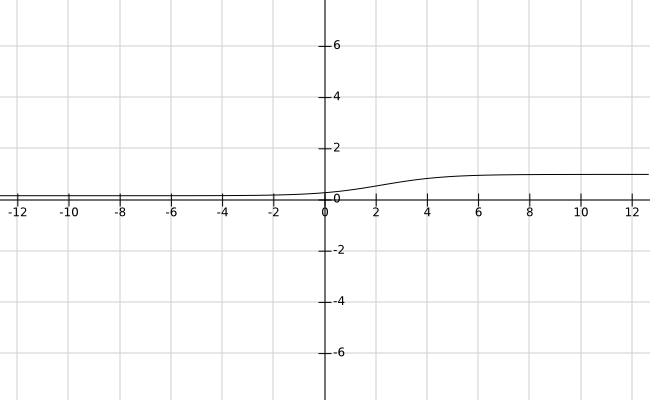
\includegraphics[scale=0.95]{q2.png}

While at it, let's also find: \\

$ P(w_2|x) = \dfrac{(\frac{2}{3})^x0.4}{ (0.6 (0.6)^x(0.4)^{1-x} + 0.4(0.4)^x(0.6)^{1-x}).\dfrac{1}{3} + (\frac{2}{3})^x0.4}  $ \\


b)  A basic decision strategy would be, choose $w_1$ is $P(w_1|x)>P(w_2|x)$, $w_2$ otherwise (We could also compare likelihood times prior, it would give the same result).

For $x=0$:\\

$P(w_1|x=0) = \dfrac{2}{7}= 0.29$ \\

$P(w_2|x=0)  = \dfrac{0.4}{0.2\cdot 0.4 + 0.4\cdot 0.2 +0.4} = 0.71 $ \\

So we choose $w_2$ (We didn't had to calculate the latter term, obviously, since the sum would have been $1$ anyway, but no harm finding it explicitly). \\

c)  $R(w_1|x=1) = \lambda_{11}P(w_1|x=1) + \lambda_{12}P(w_2|x=1) = P(w_2|x=1) $\\

$ = \dfrac{\frac{4}{5}}{0.6\cdot 0.6 + 0.4\cdot 0.4+\frac{4}{5}} = 0.606 $\\




\section*{Answer 3}
a)\\\\

$P(w_1|\bold{x}) = \dfrac{P(\bold{x}|w_1)P(w_1)}{P(\bold{x}) }  = \frac{e^{\left(-\frac{1}{2}\left(\begin{pmatrix}0.3&0.3\end{pmatrix}-\begin{pmatrix}0&0\end{pmatrix}\right)\begin{pmatrix}1&0\\ \:\:0&1\end{pmatrix}^{-1}\left(\begin{pmatrix}0.3\\ \:\:0.3\end{pmatrix}-\begin{pmatrix}0\\ \:\:0\end{pmatrix}\right)\right)}}{\sqrt{\left(2\pi \right)^2\left|\begin{pmatrix}1&0\\ \:\:0&1\end{pmatrix}\right|}} \cdot \dfrac{1}{3P(\bold{x})} = 0.12231141052 \cdot \dfrac{1}{3P(\bold{x})} = 0.04077047017 \cdot \dfrac{1}{P(\bold{x})}  $ \\\\\\

$P(w_2|\bold{x}) = \dfrac{P(\bold{x}|w_2)P(w_2)}{P(\bold{x}) }  =  \frac{e^{\left(-\frac{1}{2}\left(\begin{pmatrix}0.3&0.3\end{pmatrix}-\begin{pmatrix}1&1\end{pmatrix}\right)\begin{pmatrix}1&0\\ \:\:\:0&1\end{pmatrix}^{-1}\left(\begin{pmatrix}0.3\\ \:\:\:0.3\end{pmatrix}-\begin{pmatrix}1\\ \:\:\:1\end{pmatrix}\right)\right)}}{\sqrt{\left(2\pi \right)^2\left|\begin{pmatrix}1&0\\ \:\:\:0&1\end{pmatrix}\right|}} \cdot \dfrac{2}{3P(\bold{x})} =0.08198779033 \cdot \dfrac{2}{3P(\bold{x})}= 0.05465852688 \cdot \dfrac{1}{P(\bold{x})}  $\\\\

$P(w_3|\bold{x}) = \dfrac{P(\bold{x}|w_3)P(w_3)}{P(\bold{x}) }  = ( \frac{e^{\left(-\frac{1}{2}\left(\begin{pmatrix}0.3&0.3\end{pmatrix}-\begin{pmatrix}0.5&0.5\end{pmatrix}\right)\begin{pmatrix}1&0\\ \:\:\:0&1\end{pmatrix}^{-1}\left(\begin{pmatrix}0.3\\ \:\:\:0.3\end{pmatrix}-\begin{pmatrix}0.5\\ 0.5\end{pmatrix}\right)\right)}}{\sqrt{\left(2\pi \right)^2\left|\begin{pmatrix}1&0\\ \:\:\:0&1\end{pmatrix}\right|}}\cdot \frac{1}{2}+\frac{e^{\left(-\frac{1}{2}\left(\begin{pmatrix}0.3&0.3\end{pmatrix}-\begin{pmatrix}-0.5&0.5\end{pmatrix}\right)\begin{pmatrix}1&0\\ \:\:\:\:0&1\end{pmatrix}^{-1}\left(\begin{pmatrix}0.3\\ \:\:\:\:0.3\end{pmatrix}-\begin{pmatrix}-0.5\\ \:0.5\end{pmatrix}\right)\right)}}{\sqrt{\left(2\pi \:\right)^2\left|\begin{pmatrix}1&0\\ \:\:\:\:0&1\end{pmatrix}\right|}}\cdot \:\frac{1}{2} ) \cdot \dfrac{3}{3P(\bold{x})} = (\dfrac{0.12858245064}{2} + \dfrac{0.09525622229}{2})\cdot \dfrac{3}{3P(\bold{x})} = 0.11192 \cdot \dfrac{1}{P(\bold{x})}$\\\\

And $P(\bold{x})= 0.04077047017 + 0.05465852688 +0.11192 = 0.20734899705$\\

So we can see that, regardless of $P(\bold{x})$, the correct classification is $w_3$. \\

b)For the point (*,0.3) we just have to compare three likelihoods that are three normal distributions all with variance 1 and  means 0 1 and 0.5 respectively. It is obvious that class 3 will yield the highest probability.\\

\section*{Answer 4}

a) Let's first find the likelihood ratio, including the prior probabilities. Denote the ratio, which is a scalar, $R=R(x)$. Yet since prior probabilities are not given, we assume them to be  $0.5$ each.\\

$R(x)= \dfrac{ \dfrac{1}{\pi b}\cdot \dfrac{1}{1+(\dfrac{x-a_1}{b})^2} }{\dfrac{1}{\pi b}\cdot \dfrac{1}{1+(\dfrac{x-a_2}{b})^2}} = \dfrac{1+(\dfrac{x-a_2}{b})^2}{1+(\dfrac{x-a_1}{b})^2} = \dfrac{b^2+x^2+a_2^2-2xa_2}{b^2+x^2+a_1^2-2xa_1}$ \\

And since no loss funciton is given, we will assume unit-loss, which means we will decide $w_1$ when $R>1$ and vice-versa. So our decision boundary is $R(x)=1$. \\
 
$R(x) = 1 = \dfrac{b^2+x^2+a_2^2-2xa_2}{b^2+x^2+a_1^2-2xa_1}$ \\

Or equivalently,\\

$b^2+x^2+a_2^2-2xa_2 = b^2+x^2+a_1^2-2xa_1$ \\

$ a_2^2-2xa_2 = a_1^2-2xa_1$ \\

$x=\dfrac{a_2+a_1}{2}$ (For $a_1\neq a_2$)\\

is also the same decision boundary, independent of $b$, where $x$ is a variable and $a_1,a_2$ are constants. And our rule is now decide $w_1$ when $\dfrac{a_1+a_2}{2} > x$ and vice-versa (with the assumption that $a_2>a_1$). Without loss of generality, we can simply reverse the cases if $a_1>a_2$ . \\

The reason for all these can be shown like this:\\

We decide $w_1$ when $R>1$, or equivalently when: \\

$a_2^2-2xa_2>a_1^2-2xa_1$\\

$a_2^2-a_1^2>2xa_2-2xa_1$ \\

$(a_2+a_1)(a_2-a_1)  > 2x (a_2-a_1)$ \\

$a_2+a_1>2x$ (For $a_2>a_1$) \\

b) \\

$P(error) =\displaystyle\int_{-\infty}^{\infty}P(error|x)P(x)dx$ \\

Where $P(error|x) = min[P(w_1|x),P(w_2|x)]$. So:\\

$P(error) =\displaystyle\int_{-\infty}^{ \frac{a_1+a_2}{2} }P(w_2|x)P(x)dx + \int_{ \frac{a_1+a_2}{2}  }^{ \infty }P(w_1|x)P(x)dx $ \\

$ =\displaystyle\int_{-\infty}^{ \frac{a_1+a_2}{2} }P(x|w_2)P(w_2)dx + \int_{ \frac{a_1+a_2}{2}  }^{ \infty }P(x|w_1)P(w_1)dx $ \\
 

$ =0.5\displaystyle\int_{-\infty}^{ \frac{a_1+a_2}{2} }\dfrac{1}{\pi b}\cdot \dfrac{1}{1+(\dfrac{x-a_2}{b})^2}dx + 0.5\int_{ \frac{a_1+a_2}{2}  }^{ \infty }\dfrac{1}{\pi b}\cdot \dfrac{1}{1+(\dfrac{x-a_1}{b})^2}dx $ \\


Which when put in to a calculator, it gets evaluated to the following: \\

$\dfrac{0.5\arctan \left(\dfrac{a_1-a_2}{2b}\right)}{\pi }-\dfrac{0.5\arctan \left(\dfrac{-a_1+a_2}{2b}\right)}{\pi }+0.5\text{sgn}\left(b\right)$



\section*{Answer 5}

Say we have a model such that $Y=aX+b$. Where b is the normally distributed error. When we take the log-likelihood of $Y\mid X$ we see that the value when we try to maximiz this expression w.r.t $a$ it is the same as minimizing the error coefficient which turns out to be in the form of sum of squares.

\section*{Answer 6}
Without loss of generality, assuming each $\boldsymbol{x}$ is consisted of $1$s and $0$s, it is easy to see that;\\

$P( \boldsymbol{x} | \boldsymbol{\theta} ) = \prod_{i=1}^{d} \boldsymbol{\theta}_i^{\boldsymbol{x}_i} \cdot (1-\boldsymbol{\theta}_i)^{ 1 - \boldsymbol{x}_i } $ \\

Now, let $D=\{ \boldsymbol{x}_1,\cdots,\boldsymbol{x}_n\}$. The log-likelihood function $L$ is: \\

$L( \boldsymbol{\theta} ) = logP(D|\boldsymbol{\theta}) = log[ P(\boldsymbol{x}_1|\boldsymbol{\theta})\cdots P(\boldsymbol{x}_n|\boldsymbol{\theta})] = log\prod_{k=1}^{n} P(\boldsymbol{x}_k|\boldsymbol{\theta})  $ \\

$ = \sum_{k=1}^{n} logP(\boldsymbol{x}_k|\boldsymbol{\theta}) = \sum_{k=1}^{n} log \prod_{i=1}^{d} \boldsymbol{\theta}_i^{\boldsymbol{x_k}_i} \cdot (1-\boldsymbol{\theta}_i)^{ 1 - \boldsymbol{x_k}_i }  $ \\

$ \sum_{k=1}^{n} \sum_{i=1}^{d} log[\boldsymbol{\theta}_i^{\boldsymbol{x_k}_i} \cdot (1-\boldsymbol{\theta}_i)^{ 1 - \bold{x_k}_i }] $ \\

$ \sum_{k=1}^{n} \sum_{i=1}^{d} log[\boldsymbol{\theta}_i^{\boldsymbol{x_k}_i} ] + log[ (1-\boldsymbol{\theta}_i)^{ 1 - \boldsymbol{x_k}_i }] $ \\

$ \sum_{k=1}^{n} \sum_{i=1}^{d} \boldsymbol{x_k}_ilog[\boldsymbol{\theta}_i] + (1 - \boldsymbol{x_k}_i)log[1-\boldsymbol{\theta}_i] $ \\

Now, let's take derivative of $L(\boldsymbol{\theta})$ w.r.t $\boldsymbol{\theta}$. Since our $L$ is not in vector notation, we can separately take partial derivative w.r.t to $\boldsymbol{\theta}_j$ and find their LMEs separately. \\

Notice that the inner summation's terms will be zero, when we take partial derivative, when $i\neq j$.\\

$\dfrac{\varphi L}{\varphi \boldsymbol{\theta}_j} =  \sum_{k=1}^{n} \boldsymbol{x_k}_j \dfrac{1}{\boldsymbol{\theta}_j} + (1 - \boldsymbol{x_k}_j)\dfrac{-1}{1-\boldsymbol{\theta}_j} = 0$ \\

$ \sum_{k=1}^{n} \boldsymbol{x_k}_j \dfrac{1}{\boldsymbol{\theta}_j} = \sum_{k=1}^{n} (1 - \boldsymbol{x_k}_j)\dfrac{1}{1-\boldsymbol{\theta}_j} $ \\

$ \sum_{k=1}^{n} \boldsymbol{x_k}_j \dfrac{1}{\boldsymbol{\theta}_j} = \sum_{k=1}^{n} \dfrac{1}{1-\boldsymbol{\theta}_j} - \dfrac{\boldsymbol{x_k}_j}{1-\boldsymbol{\theta}_j} $ \\


$ \sum_{k=1}^{n} \boldsymbol{x_k}_j - \boldsymbol{x_k}_j
 \boldsymbol{\theta }_j = \sum_{k=1}^{n} \boldsymbol{\theta}_j - \boldsymbol{\theta}_j \boldsymbol{x_k}_j $ \\
 
 $ \sum_{k=1}^{n} \boldsymbol{x_k}_j  = \sum_{k=1}^{n} \boldsymbol{\theta}_j = n\boldsymbol{\theta}_j $ \\
 
 $ \dfrac{1}{n} \sum_{k=1}^{n} \boldsymbol{x_k}_j  = \boldsymbol{\theta}_j $ \\
 
 is the best estimate for $\boldsymbol{\theta}_j$. Since the same can be shown for each $j$, we can generalize this to the following vector notation:
 
 $ \boldsymbol{\hat{\boldsymbol{\theta}}} = \dfrac{1}{n} \sum_{k=1}^{n} \boldsymbol{x_k}   $
 
 Which was what wanted to be showed.



\section*{Answer 7}

The given equation is just going to become $\frac{1}{n}(X-\mu )(X-\mu )^{T}$ which is basically just $\frac{1}{n}\begin{bmatrix}
    x_{1}-\mu_{1}\\
    \vdots\\
     x_{n}-\mu_{n}
\end{bmatrix}
$
$\begin{bmatrix}
    x_{1}-\mu_{1}
    \cdots
     x_{n}-\mu_{n}
\end{bmatrix}
$ The result of this vector mıltiplication becomes a \\matrix where the i,jth entry is $x_{i}-\mu_{i}x_{j}-\mu_{j}$ which is basically $Cov(x_{i},x_{j})$ which means we have attained the covariance matrix.


\section*{Answer 8}

\quad Let us define $D=\{\bold{x_1},\cdots\bold{x_n}\}$ where each $\bold{x_i}\in R^d$. \\

In a MAP we will try to maximize $P(D|\boldsymbol{\mu}) P(\boldsymbol{\mu}) $.\\

Note that: \\

$P( \boldsymbol{x} | \boldsymbol{\mu} ) = \dfrac{1}{(2\pi)^{d/2}|\bold \Sigma|^{1/2}}exp(-\dfrac{1}{2}(\bold{x}-\boldsymbol{\mu})^T)  \Sigma^{-1} (\bold{x}-\boldsymbol{\mu})) $ \\

Also, let us define, \\

$a= \dfrac{1}{(2\pi)^{n/2}|\Sigma|^{1/2}}$\\

Which is a scalar independent of $\boldsymbol{\mu}$\\.

And the prior is:\\

$P(\bold{\mu})  = \dfrac{1}{(2\pi)^{d/2}|\bold{\Sigma}_0|^{1/2}}exp(-\dfrac{1}{2}(\boldsymbol{\mu}-\boldsymbol{\mu}_0)^T  \bold\Sigma_0^{-1} (\boldsymbol{\mu}-\boldsymbol{\mu}_0)) $ \\

Also, let us define, \\

$b= \dfrac{1}{(2\pi)^{n/2}|\bold{\Sigma}_0|^{1/2}}$\\

And in our book Pattern Classification section 3.2.2 equation 9, it is given that;\\

$lnP(\bold{x}|\bold{\mu})= -\dfrac{1}{2}ln[(2\pi)^d|\Sigma|]-\dfrac{1}{2}(\bold{x}-\boldsymbol{\mu})^T\Sigma^{-1}(\bold{x}-\boldsymbol{\mu}) $\\

 The log-likelihood function $L$ is: \\

$L( \boldsymbol{\mu} ) = ln(P(D|\boldsymbol{\mu})P(\boldsymbol{\mu}))  = ln[ P(\boldsymbol{x}_1|\boldsymbol{\mu})\cdots P(\boldsymbol{x}_n|\boldsymbol{\mu})P(\boldsymbol{\mu})  ] = ln[(\prod_{k=1}^{n} P(\boldsymbol{x}_k|\boldsymbol{\mu}))P(\boldsymbol{\mu}) ]   $ \\

$ = \sum_{k=1}^{n} lnP(\boldsymbol{x}_k|\boldsymbol{\mu})P(\boldsymbol{\mu})  $\\

$ = [\sum_{k=1}^{n} ln(a)-\dfrac{1}{2}(\bold{x_k}-\boldsymbol{\mu})^T\bold\Sigma^{-1}(\bold{x_k}-\boldsymbol{\mu}) ]+ ln(b) -\dfrac{1}{2}(\bold{\mu}-\boldsymbol{\mu}_0)^T\bold\Sigma_0^{-1}(\boldsymbol{\mu}-\boldsymbol{\mu}_0) $\\

Now, let's take derivative of $L$ and equate to zero:\\

$ \dfrac{dL}{d\boldsymbol\mu}  = [\sum_{k=1}^n \bold \Sigma^{-1}(\bold x_k-\boldsymbol\mu)]-\bold\Sigma_0^{-1}(\boldsymbol\mu-\boldsymbol\mu_0) = 0$\\

$ \sum_{k=1}^n \bold \Sigma^{-1}(\bold x_k-\boldsymbol\mu)=\bold\Sigma_0^{-1}(\boldsymbol\mu-\boldsymbol\mu_0) $\\

$ \sum_{k=1}^n  \bold \Sigma^{-1}\bold x_k-n\bold \Sigma^{-1}\bold\mu= \bold\Sigma_0^{-1} \boldsymbol\mu-
\bold\Sigma_0^{-1}\boldsymbol\mu_0 $\\

$\bold\Sigma_0^{-1}\boldsymbol\mu_0 + \bold \Sigma^{-1}\sum_{k=1}^n  \bold x_k = \bold\Sigma_0^{-1} \boldsymbol\mu + n\bold \Sigma^{-1}\bold\mu = (\bold\Sigma_0^{-1} + n\bold \Sigma^{-1} ) \bold\mu $\\

So; \\

$\hat{\bold\mu} = \dfrac{\bold\Sigma_0^{-1}\boldsymbol\mu_0 + \bold \Sigma^{-1}\sum_{k=1}^n  \bold x_k }{(\bold\Sigma_0^{-1} + n\bold \Sigma^{-1} ) } $\\

Is our MAP estimator.  \\

b) First let's find the transformed values;

$\boldsymbol\mu'=E(\bold x')=E(\bold A \bold x) = \bold A E(\bold x) = \bold A \boldsymbol\mu$ \\

and \\

$\bold \Sigma' = E[(\bold x' - \boldsymbol \mu') (\bold x' - \boldsymbol \mu')^t] $\\

$= E[(A\bold x - A\boldsymbol \mu) (A\bold x - A\boldsymbol \mu)^t] $\\

$= E[\bold A(\bold x - \boldsymbol \mu) (\bold x - \boldsymbol \mu)^t\bold A^t] $\\

$= \bold AE[(\bold x - \boldsymbol \mu) (\bold x - \boldsymbol \mu)^t]\bold A^t $\\

$= \bold A\bold\Sigma \bold A^t $\\

Now,even tough the question lacks a definition for what is an "appropriate estimate", we can try recalculating MAP  for the transformed space. We need to find $P(\bold x' | \bold \mu')$ and a new prior $P(\bold\mu')$ \\


$P( \boldsymbol{x'} | \boldsymbol{\mu'} ) = \dfrac{1}{(2\pi)^{d/2}|\bold\Sigma'|^{1/2}}exp(-\dfrac{1}{2}(\bold{x'}-\bold{\mu'})^T) \bold \Sigma'^{-1} (\bold{x'}-\bold{\mu'})) $ \\

$ =  \dfrac{1}{(2\pi)^{d/2}|\bold A \bold\Sigma\bold A^t|^{1/2}}exp(-\dfrac{1}{2}(\bold A \bold{x}-\bold A \bold{\mu})^T  (\bold  A^t)^{-1}  \bold \Sigma^{-1} \bold A^{-1} (\bold A \bold{x}- \bold A \boldsymbol{\mu})) $ \\

$ =  \dfrac{1}{(2\pi)^{d/2}|\bold A \bold\Sigma\bold A^t|^{1/2}}  exp(-\dfrac{1}{2}(\bold{x}-\boldsymbol{\mu})^T  \bold A^t (\bold  A^t)^{-1}  \bold \Sigma^{-1} \bold A^{-1} \bold A (\bold{x}- \bold{\mu})) $ \\

$ = \dfrac{a}{  |\bold A \bold A^t|^{1/2} }exp(-\dfrac{1}{2}(\bold{x'}-\boldsymbol{\mu'})^T) \bold \Sigma'^{-1} (\bold{x'}-\boldsymbol{\mu'})) $ \\

Remember how we defined $a$ from part (a). The derivation will be the same for $P(\bold{\mu}) $:


$P(\boldsymbol{\mu})  = \dfrac{b}{  |\bold A \bold A^t|^{1/2} }exp(-\dfrac{1}{2}(\bold{\mu}-\bold{\mu}_0)^T  \bold\Sigma_0^{-1} (\bold{\mu}-\bold{\mu}_0)) $ \\

So by the transformation of the space, we only scaled the constants $a$ and $b$. It is easy to see that our new log-likelihood $L(\bold\mu)$ will be:

$L(\boldsymbol\mu) = [\sum_{k=1}^{n} ln(\dfrac{a}{  |\bold A \bold A^t|^{1/2} })-\dfrac{1}{2}(\bold{x_k}-\bold{\mu})^T\bold\Sigma^{-1}(\bold{x_k}-\bold{\mu}) ]+ ln(\dfrac{b}{  |\bold A \bold A^t|^{1/2} }) -\dfrac{1}{2}(\bold{\mu}-\bold{\mu}_0)^T\bold\Sigma_0^{-1}(\bold{\mu}-\bold{\mu}_0) $\\

And when we take the derivative, these scaled terms of $a$ and $b$ will vanish, since they are just constants. The final MAP estimator will be the same as the old one:

$\hat{\boldsymbol\mu'}  = \hat{\boldsymbol\mu} = \dfrac{\bold\Sigma_0^{-1}\boldsymbol\mu_0 + \bold \Sigma^{-1}\sum_{k=1}^n  \bold x_k }{(\bold\Sigma_0^{-1} + n\bold \Sigma^{-1} ) } $\\


So it turns out, yes, our old MAP estimator gives an appropriate estimate for the transformed space.




%The question basically asks whether our prior density is "non-informative" w.r.t transformation A. This can be formally stated as whether or not the following holds; \\

%$P(\bold\mu) =^? AP(A^{-1}\bold\mu) $ \\

%Let's check; \\

%$ AP(A^{-1}\bold\mu)  =^? \dfrac{A}{(2\pi)^{d/2}|\bold{\Sigma}_0|^{1/2}}exp(-\dfrac{1}{2}(A^{-1}\bold{\mu}-\bold{\mu}_0)^T  \bold\Sigma_0^{-1} (A^{-1}\bold{\mu}-\bold{\mu}_0)) $ \\

%Well, it is obvious that our prior will not hold for such constraint. So no, our MAP estimator will not give the appropriate estimate for the transformed mean $\mu'$.




\section*{Answer 9}


a)We use the linearity of expectation to show that $ E[\hat{\mu}]=\frac{1}{n}(E[x_{1}]+E[x_{2}]+E[x_{3}]+...+E[x_{n}])$ which is $x_{1}=\frac{n\cdot x_{1}}{n}$ so the estimator is unbiased
b)The ML estimate for $\hat{\mu}$ is $\frac{x_{1}+x_{2}+...+x_{n}}{n}$ which maskes the variance $\hat{\sigma}=\sum_{i} x_{i}-\hat{\mu}$ for the mean in part a we would have a zero term which would distort the variance undesirably.\\
c)Again we use the linearity of expectation $(n-1)E[\hat{\sigma}]$=$E[\sum_{i=1}^{n}x_{i}^{2}-2\mu x_{i} +\mu^{2}]$\\
Which will obiously become $(n-1)E[\hat{\sigma}]$=$n(E[x_{i}^{2}]-E[\mu^{2}])$ which is $\frac{n-1}{n} E[\hat{\sigma}]$=$(E[x_{i}^{2}]-E[\mu^{2}])$







\section*{Answer 10}


% Please add the following required packages to your document preamble:
% \usepackage{graphicx}
\begin{table}[]
\resizebox{\textwidth}{!}{%
\begin{tabular}{l|l|l|l}
                 & Gaussian                                                                                                                                                                                                                                                                                                                                                                                                                                                                & Cauchy                                                                                                                                                                                                                                                                             & Uniform                                                                                                                                                                                                                                                                                                       \\ \hline
Random Sample    & \begin{tabular}[c]{@{}l@{}}This is an overall bad estimator\\ for gaussian, yet since the \\ samples closer to the mean are\\ more likely to be selected \\ (and even to be sampled in the\\ first place),gaussian is the \\ most appropriate for this kind \\ of sampling out of three.\end{tabular}                                                                                                                                                                   & \begin{tabular}[c]{@{}l@{}}Same as Gaussian, the only difference\\ is that for Cauchy this sampling is \\ sligthly worse since the tails are fatter \\ and the middle bell is thinner compared to \\ gaussian, so sampling closer to mean is a \\ little less likely.\end{tabular} & \begin{tabular}[c]{@{}l@{}}Uniform is the worst distribution for\\  this sampling since all values regardless\\  of their distances to mean are equally\\  likely to be selected.\end{tabular}                                                                                                                \\ \hline
Avg. of Samples  & \begin{tabular}[c]{@{}l@{}}This is a good estimator for \\ all of them, satisfying many \\ wanted properties, and also \\ coincides with some know estimators.\end{tabular}                                                                                                                                                                                                                                                                                             & -                                                                                                                                                                                                                                                                                  & -                                                                                                                                                                                                                                                                                                             \\ \hline
Avg. of Extremes & \begin{tabular}[c]{@{}l@{}}This is an ok estimate, since\\ the distrubution is symetric\\ around mean. Yet comparing\\ between three, this is most\\ apropriate for the uniform\\ case, since it is more likely\\ that the choosen extremes will\\ have the same distance from\\ mean. For gaussian and cauchy,\\ since they have tails, it is more\\ likely that one extreme "over-throws" \\ the other one, which means is further\\ away from the mean.\end{tabular} & \begin{tabular}[c]{@{}l@{}}As always, cauchy is between uniform \\ and gaussian w.r.t how much helpfull \\ this sampling method is.\end{tabular}                                                                                                                                   & -                                                                                                                                                                                                                                                                                                             \\ \hline
Trimmed Mean     & \begin{tabular}[c]{@{}l@{}}This method helps for gaussian,\\ since both gaussian and cauchy\\ has tails which means for a\\ small chance a very big or\\ small sample may impact the\\ average disproportionally.\\ By trimming, we reduce the\\ chance of this happening.\end{tabular}                                                                                                                                                                                 & -                                                                                                                                                                                                                                                                                  & \begin{tabular}[c]{@{}l@{}}For uniform tough i believe this \\ does not make a difference when \\ compared with Avg. of Samples. Since \\ The trimmed values are equally likely \\ to appear compared to non-trimmed values, \\ intiutively speaking this doesn't \\ change our "sampling bias".\end{tabular}
\end{tabular}%
}
\end{table}


\section*{Answer 11}

a)If we take the limit of both equations as they go to infinity we see that $\mu_{n}$ approaches $\hat{\mu_{n}}$. We see that the coefficient of the first term approaches 1 as the denominator of the second term goes to infinity making the coefficient 0. For $\sigma_{n}^{2}$ approaches 0, since again the denominator will outgrow the expression, this makes quite a lot of sense since as the sample size increases it is bound to be more predictable.\\
b)The limit of $\mu_{n}$ as n approaches 0 is $\mu_{0}$. Since we know the limit at infinity which is $\hat{\mu_{n}}$, we can easily say that $\mu_{n}$ lies between these two.\\
c)So basically $\sigma^{2}_{0}$=0 which makes $\mu_{n}$=$\mu_{0}$ and $\sigma_{n}^{2}$=0. İt also means that we have guessed the parameters of the distribution exactly. Which is why neither $\sigma_{n}^{2}$ nor $\mu_{n}$ will not change as the sample size grows\\
d)$\mu_{n}$ becomes $\hat{\mu_{n}}$, and $\sigma_{n}^{2}$ becomes $\frac{\sigma^{2}}{n}$

\section*{Answer 12}





\end{document}


